\documentclass{article}
\usepackage[utf8]{inputenc}
\usepackage{graphicx}

\title{Operating Systems Notes}
\author{Jacob Burley} %add your name here if you're a collaborator
\date{12 December 2017}

\begin{document}
%images aren't working for whatever reason (pdflatex doesn't find them at build time) which I think requires some extra configuration but the images aren't as important as the content so that's not a focus for me at the moment

\maketitle
\section{Introduction}
Operating System runs in kernel mode (supervisor mode), User programs run in User Mode
\\Instructions that control the machine or us I/O aren't available to User Mode (at least not directly)
%\\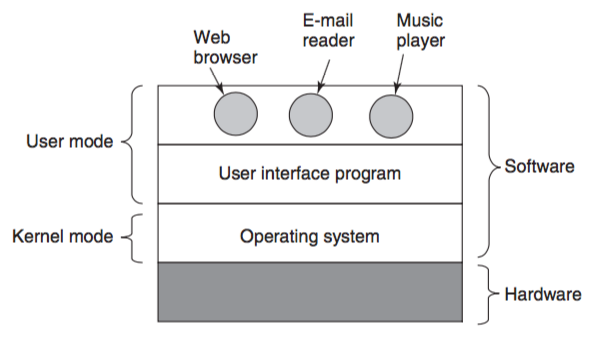
\includegraphics[width= 250pt]{tex/ch1/1-1.png}
\\Operating System runs on bare hardware
\\OS extends hardware of a computer, and makes it easier for programmers to develop applications without having to deal with things like SATA interfaces directly
\\OS also provides abstractions for devices, files etc.
%\\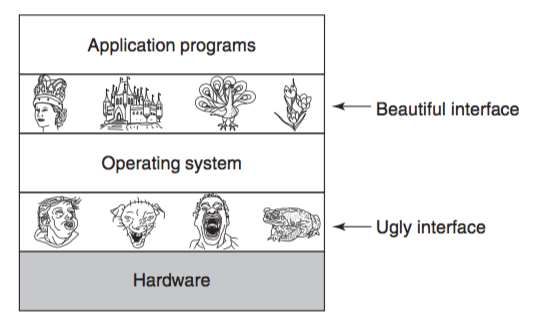
\includegraphics[width = 250pt]{tex/ch1/1-2.png}
\\OS also manages hardware resources like CPU and RAM, as well as I/O
\\Earliest (first generation) computers didn't have an OS, were manually programmable using absolute machine language or physically rewiring plugboards to control basic functions of the machine
\\Second generation machines used transistors, became much more reliable
\\Batch systems involved collecting jobs on punchcards, reading them onto magnetic tape using a dedicated machine for this purpose, using this magnetic tape as input on the main computing machine, and then taking the output tape of that machine to another dedicated machine that printed the contents of the output tape
\\Structure of input job
\begin{itemize}
	\item \$JOB card, specifies maximum runtime in minutes, account number to be charged and programmer name
	\item \$FORTRAN card tells machine to load the FORTRAN compiler from the system tape, directly followed by program to be compiled
	\item \$LOAD card directed machine to load the object program that was just compiled
	\item \$RUN card, telling machine to run the program with the data that followed (like run-time arguments)
	\item \$END card marks the end of a job
\end{itemize}
\section{Processes & Threads}

\section{Memory Management}

\section{File Systems}

\section{I/O}

\section{Deadlocks}

\end{document}